\documentclass[12pt, letterpaper]{article}
\usepackage[titletoc,title]{appendix}
\usepackage{color}
\usepackage{booktabs}
\usepackage[usenames,dvipsnames,svgnames,table]{xcolor}
\definecolor{dark-red}{rgb}{0.75,0.10,0.10}
\definecolor{dark-blue}{rgb}{0.0,0.0,0.7}
\usepackage[margin=1in]{geometry}
\usepackage[linkcolor=dark-blue,
			colorlinks=true,
			urlcolor=blue,
			pdfstartview={XYZ null null 1.00},
			pdfpagemode=UseNone,
			citecolor={dark-blue},
			pdftitle={Propagation of Error}]{hyperref}
%\usepackage{biblatex}
\usepackage{multibib}
\newcites{sec}{Other Sources}
\usepackage{geometry} % see geometry.pdf on how to lay out the page. There's lots.
\geometry{letterpaper}               % This is 8.5x11 paper. Options are a4paper or a5paper or other...
\usepackage{graphicx}                % Handles inclusion of major graphics formats and allows use of
\usepackage{amsfonts,amssymb,amsbsy}
\usepackage{amsxtra}
\usepackage{natbib}
\usepackage{dcolumn}
\usepackage{longtable}
\usepackage{verbatim}
\setcitestyle{round,semicolon,aysep={},yysep={;}}
\usepackage{setspace}		     % Permits line spacing control. Options are \doublespacing, \onehalfspace
\usepackage{sectsty}		     % Permits control of section header styles
\usepackage{lscape}
\usepackage{fancyhdr}		     % Permits header customization. See header section below.
\usepackage{url}                     % Correctly formats URLs with the \url{} tag
\usepackage{fullpage}		%1-inch margins
\usepackage{multirow}
\usepackage{rotating}
\setlength{\parindent}{3em}

\usepackage{float}

\usepackage[T1]{fontenc}
\usepackage{bm}
\usepackage{libertine}
\usepackage{dcolumn}
\usepackage{chngcntr}

% Caption
\usepackage[hang, font=small,skip=0pt, labelfont={bf}]{caption}
\captionsetup[subtable]{font=small,skip=0pt}
\usepackage{subcaption}

% tt font issues
% \renewcommand*{\ttdefault}{qcr}
\renewcommand{\ttdefault}{pcr}

\usepackage{lscape}
\renewcommand{\textfraction}{0}
\renewcommand{\topfraction}{0.95}
\renewcommand{\bottomfraction}{0.95}
\renewcommand{\floatpagefraction}{0.40}
\setcounter{totalnumber}{5}
\makeatletter
\providecommand\phantomcaption{\caption@refstepcounter\@captype}
\makeatother
\begin{comment}

setwd(paste0(githubdir, "propagation_of_error/ms/"))
tools::texi2dvi("error.tex", pdf = TRUE, clean = TRUE)
setwd(githubdir)

\end{comment}

\begin{document}
\title{\Large{Propagation of Error: Citations\\ to Problematic Research}\footnote{We are grateful to Danielle Portnoy and Xiaoran Huang for assisting us with the research, and to Andrew Gelman, Kabir Khanna, and Daniel Stone for offering valuable comments. The data and scripts for replicating the analysis are posted at: \href{https://github.com/recite/propagation_of_error}{https://github.com/recite/propagation\_of\_error}}\\\vspace{5mm}}

\author{Ken Cor\\
\and Gaurav Sood}
%\vspace{5mm}}
%\date{\normalsize{\today}}
\maketitle

\vspace{.2cm}
\doublespacing
\clearpage
%\renewcommand{\abstractname}{Summary}
%\begin{abstract}
\textbf{Summary.} To shed light on how often scientists base their claims on problematic research, we exploit data on cases where problems with research are broadly publicized. Using data from over 3,000 retracted articles and over 74,000 citations to these articles, we find that at least 31\% of the citations to retracted articles happen a year after they have been retracted and that about 91\% of the post-retraction citations note no concern with the cited article. We augment the analysis with data from an article published in \textit{Nature Neuroscience}, highlighting a serious statistical error in articles published in prominent journals. Data suggest that problematic research was cited without noting concerns with the work \textit{more frequently} after the problem was publicized.
\vspace{.2cm}\\
\singlespacing
%\end{abstract}
\textit{Keywords.} Citation Behavior, Retractions, Scientific Integrity, Scientific Misconduct, Scientometrics
\doublespacing
\clearpage

\section{Introduction}

Citations are the bedrock of the scientific process. Scientists use citations to give credit for being first (``$x$, $y$, and $z$ have studied $a$''), to debate methods and inferences (``the method used in study $x$ fails to account for $s$''), as evidence (``$x$ shows $a$'', ``we use data from $x$ for our meta-analysis''), and to contextualize results (``our results are consistent with results from $y$''). And unless the researcher notes problems with cited research, citations cue that the data, results, inferences, or in some cases, the entire article, can be trusted.

When researchers cite articles with serious errors without acknowledging the errors, problems ensue. When erroneous research is cited as evidence \citep[e.g.,][]{chang2013safety, torsvik2010spontaneous}, it cues that the evidence for the claim is good. Such citations unduly increase the reader's confidence in the result or argument. In the extreme, a reader may become persuaded that the point being buffeted by a citation to problematic research is right. The reader, generally another academic, may go on to write other articles influenced by the incorrect point, citing the erroneous article for support, or may share the point as fact with colleagues, students, and practitioners, propagating the error.

For example, consider an article published in April 2005 by \citet{rubio2005spontaneous} reporting a disturbing finding in \textit{Cancer Research}. They report discovering that stem cells can spontaneously transform into cancerous cells during \textit{in vitro} experiments. The finding was a blow to research in the use of stem cells to treat cancer. By 2010, according to \textit{Web of Science}, the article had been cited over 300 times.

In August 2010, the article was retracted \citep{de2010retraction}. The authors had been unable to replicate the result, and there was mounting evidence that transformations like the one reported were due to a basic error: cross-contamination during cell culturing. While this episode can be seen in a favorable light given that the errors were caught and a retraction notice was issued, the story does not end there.

Since 2010, the article has been cited another 300 plus times, with most citations noting no concern with the original work. For instance, a year after being retracted, \citet{firinci2011mesenchymal} published an article in \textit{International Immunopharmacology} citing \citeauthor{rubio2005spontaneous} as basis for warning scientists that stem cells can spontaneously transform. Two years after the retraction, \citet{kosaka2012therapeutic} published an article in \textit{Cancer Gene Therapy} in which they cited the evidence from \citeauthor{rubio2005spontaneous} as a hurdle to implementation of the treatment they found to be effective. Three years after the retraction, \citet{chang2013safety} published an article in \textit{Aesthetic Plastic Surgery} citing \citeauthor{rubio2005spontaneous} to argue that spontaneous transformation of human stem cells remains a risk.

Citing erroneous research without acknowledging errors is problematic in other ways. Such citations give full credit to research (and researchers) when at best partial credit is deserved. And since citation tallies cue credibility, such citations make erroneous research appear yet more credible.

Lastly, sometimes research with serious errors is cited to acknowledge the source of the data. For instance, \citet{lin2013perioperative} used data from ``two retracted studies ... without acknowledgment of their retractions, both of which were for fraudulent data...'' \citep[p. 1,][]{paul2015comment} in a meta-analysis. In such cases, the consequence is obvious and extreme---the key findings in the published work are incorrect.

In this paper, we study how common citations to problematic research that do not note concerns with the original work are.

\section{Citations to Problematic Research}

The problem of citing problematic research without noting the problems takes special urgency in light of two empirical findings.  First, the number of retractions---research where the problems are serious enough to warrant a retraction---is rising, even after controlling for the number of articles published \citep{grieneisen2012comprehensive, steen2011retractions}.\footnote{\citet{steen2013has} posits that the rise in retractions is a result of declining quality of research and better ability to detect problems.} Second, the main reasons research is retracted---major error and fraud---are concerning \citep{bozzo2017retractions, grieneisen2012comprehensive,  singh2014comprehensive}.

Because of these reasons, researchers have started to look at how citation rates change post retraction \citep{bar2018temporal, rubbo2019citation} and whether citations post retraction acknowledge problems in the retracted work \citep[e.g.,][]{bar2017post, hamilton2019continued, luwel2018schon}. \citet{bar2018temporal}, for instance, use a sample of 994 retracted articles from \texttt{ScienceDirect} from a single month---October 2014---and find that the total number of citations to retracted articles grew over time. Similarly, \citet{rubbo2019citation} use a sample of 238 retracted engineering articles and their citations and report the number of times the articles are cited pre and post retraction and find no apparent difference. Neither article notes whether citations after retraction note problems with the cited article. Some studies, however, consider whether post retraction citations acknowledge problems. \citet{bar2017post}, for instance, find that, of the 283 citations to retracted case-study articles, a majority did not note problems with the article they cited. Similarly, \citet{hamilton2019continued} report that of 358 citations to retracted articles in the radiation oncology field, 92\% referenced the research as legitimate. Finally, \citet{luwel2018schon} studied pre- and post- retraction citations to a set of highly publicized retractions and found that over 95\% of citations were positive or neutral in how the researchers characterized the cited work. Older research has found similar results. A study using a database of 235 retracted biomedical articles found that nearly 94\% of the citations after retraction treated research as valid \citep{budd1998phenomena} and work done as far back as 1990, exploiting a dataset of 82 retracted articles, came to similar conclusions \citep{pfeifer1990continued}.

While these studies consistently show high rates of positive or neutral citations to retracted research following retraction, they all use small samples or samples that span a single discipline. The use of small, selective samples means that we cannot confidently say how widespread the problem is. With the exception of \citet{luwel2018schon}, the work also focuses on citations after retraction, which means that we cannot say how common citations that fail to acknowledge concerns are before the problems are publicized and if the rate changes after publicity.

As we note above, retractions are generally a result of serious scientific malpractice. Retractions are also easily identified. Because of these reasons, research on citations to problematic research focuses exclusively on citations to articles that have been officially retracted. However, by focusing on retractions alone, we miss the more common problem of citations to unretracted studies with major errors. For example, \citet{gelman2006} discuss a common statistical error where researchers treat differences between significant and non-significant results as significant without conducting the requisite statistical test. They describe a scenario where results from two independent studies report parameter estimates and standard errors of 25 $\pm$ 10 and 10 $\pm$ 10, respectively. The first result is significant at the 1\% level, while the second is non-significant. The finding is interpreted by many as evidence of a significant difference, but a basic calculation of the difference in the effects and its standard error tells a different story, $15 \pm \sqrt{10^{2} + 10^{2}}$, which is not significant at the conventional 95\% level.

\citet{nieuwenhuis2011} analyzed 157 behavioral, systems, and cognitive neuroscience articles that relied on such analysis and were published in journals like \textit{Nature}, \textit{Science}, \textit{Neuron}, and \textit{Journal of Neuroscience} between 2009 and 2010. They found that roughly half (79) of the articles made this error. Further, they found that the error had serious consequences for the results for approximately two-thirds of the studies that made the error. To date, none of the studies that \citet{nieuwenhuis2011} identified as problematic have been retracted. We assess whether the citation rate changes after the publication of \citet{nieuwenhuis2011}.

In all, there is growing evidence that retracted research continues to be cited long after being retracted. Most of the evidence comes from studies that use small, selective samples. Moreover, the studies present data on post retraction citations than the change in number and quality of citations after a retraction. In all, there is little research on how the quality and quantity of citations change after a retraction. Further, there is no study that we know of that studies how citations to unretracted research with serious errors changes after errors are identified by means other than a retraction. In this paper, we bridge these gaps by exploiting a large dataset of retracted articles and citations to these articles and articles used by \citet{nieuwenhuis2011}.

\section{Methods}

\subsection{Hypotheses and Research Design}

We expect the publication of the retraction notice to raise awareness about the retracted article. We also expect an article noting a potentially serious error to increase awareness about the error. Both should reduce citations to problematic research, especially citations that fail to acknowledge the problem.

We also expect the decline in citations due to publicity about a general error to be more tepid than the decline due to a retraction. For one, retractions are unequivocal indicators of serious problems with an article. For two, retractions elicit a response from the publishers, who often switch titles of the retracted articles in their online databases to reflect that they have been retracted. For three, retractions are tied to specific articles. To find out articles affected by the error highlighted in an article, e.g., \citet{nieuwenhuis2011}, scientists need to read the article they cite closely.

Formally, we hypothesize that:
\begin{enumerate}
	\item Retracted articles will receive fewer citations per year after the retraction, controlling for the time trend in citations.
	\item Articles identified by \citet{nieuwenhuis2011} as suffering from a general statistical error will receive fewer citations per year after the publication of  \citet{nieuwenhuis2011} vis-a-vis similar articles without the error.
\end{enumerate}

To estimate the impact of the publication of error on citation rates, we implement an event study design by tracking the citation rate a few years before and after the error is made public. Given long publication cycles and assuming the article would have been accepted for publication before the discovery of the error, we test the impact on citations one, two, and three years after the publication of the retraction notice. For \citet{nieuwenhuis2011}, we also use a Difference-in-Differences estimator, exploiting the fact that roughly half of the articles published in the same journals did not make the same error. 

\subsection{Data}

Our first dataset contains over 3,000 retracted articles and nearly 74,000 citations to the retracted articles extracted from the \href{https://webofknowledge.com}{Web of Science} (WoS) database \citep{clarivate2016web}. The second dataset is the set of articles identified by \citet{nieuwenhuis2011} that mistake the difference between a statistically significant and statistically insignificant result as evidence that the difference is statistically significant.

We used WoS to assemble the set of 3,000 retracted articles and over 74,000 citations because it is one of the most comprehensive curated databases of academic research from all disciplines. WoS indexes articles from over 9,500 natural science journals and 3,500 social science journals \citep{yong2013web}. WoS indexes articles from over 12,000 international journals and 148,000 conferences \citep{yong2013web}. WoS contains key citation indices including the \textit{Science Citation Index Expanded} (over 9,500 journals; 1900--present), \textit{Social Sciences Citation Index} (over 3,500 journals; 1900--present), \textit{Arts \& Humanities Citation Index} (over 1,700 journals; 1975--present), \textit{Conference Proceedings Citation Index} (over 170,000 conferences; 1990-present), \textit{Book Citation Index} (over 30,000 titles; 2005--present), among others. For a full list of titles included in the \textit{Science Citation Index Expanded}, \textit{Social Sciences Citation Index}, \textit{Arts \& Humanities Citation Index}, and \textit{Conference Proceedings Citation Index}, and a synopsis of the \textit{Book Citation Index}, see \href{https://github.com/recite/propagation\_of\_error/tree/master/data/11\_wos/what\_is\_in\_wos/}{here}. Most importantly for our work and unlike freely available databases like Google Scholar, WoS offers a way to filter results based on correction flags as well as the ability to download standardized article records containing extensive metadata.

To build a database of retracted articles, we started by creating a list of retraction notices. To do that, in August 2016, we searched WoS for titles containing the phrase ``retraction of.'' The search yielded more than 14,000 records. Using the ``corrections'' filter in WoS---it is a WoS flag for retraction and correction notices---we filtered the list to 4,085 retraction notices.

Next, we wrote software to automatically search the WoS database for retracted articles using the information in the retraction notice records. Retraction notice records did not contain consistent titles to allow a simple search, but 99\% of the retraction notices contained the year the original article was published, and 96\% listed the authors of the original work. We used these two pieces of information along with the name of the publication to search the WoS for the original articles. The search resulted in a list of 3,776 articles. We could not locate the remaining 309 retracted articles.

Due to the variability in the information contained in the retraction notice records, the automated search process returned the wrong article in some cases. Our aim was to have zero false positives, even at the risk of some false negatives. With that aim, we created rules to flag potential false positives. First, if the list of authors of the retracted article did not match the list of authors for the relevant retraction notice record, we flagged the record as a potential false positive. Second, if the title of the retracted article did not contain the words ``retracted'' or ``retraction,'' we flagged it as a potential false positive.\footnote{Our data suggests that it has become common practice for titles of original articles to be revised to indicate that the article has been retracted. However, adherence may vary across disciplines. As a result, our sample may be biased in favor of disciplines where the adherence is greater.} Third, we parsed the title of the retracted notices to extract the title of the original retracted article, and we flagged articles where the titles did not match as potential false positives. We then reviewed the potential false positives, filtering out all records where we could not verify the match. This resulted in a set of 3,084 articles. Finally, we checked for duplicates. We found 55. This left us with 3,029 articles that served as our final sample.\footnote{As an additional robustness check, we manually checked a random sample of 100 retracted articles to confirm that the article had indeed been retracted. We found that all of them were.}

To get a list of citations to these articles, we used the WoS functionality that allows users to access the list of citations to articles. We wrote software to download citation records for each of the retracted articles automatically. In total, we found 73,564 citations. Our final dataset has 3,029 retracted articles and 73,564 citations to the retracted articles. We used a similar process to access and download citation records to all 170 articles identified by \citet{nieuwenhuis2011} from WoS to create the second dataset.

\section{Results}
\subsection{Evidence From Citations to Retracted Articles}
Table ~\ref{tab:recite_ret_sum} presents some descriptive statistics about the WoS data. The first column contains data on retracted articles and the second column presents data on articles that cite the retracted articles. On average, retracted articles have been cited about 31 times in total, the average impact factor in which they were published is a striking 6, and by 2016, it had been about nine years on average since they were published. We do not have data on the average number of citations received by articles that cited the retracted articles. On average, the articles citing the retracted articles were published in less prestigious journals, with an average impact factor of about 5. And expectedly, the articles citing the retracted articles are a bit newer---they had closed close to 7 years by 2016 on average. 

To describe the fields in which retractions occur, we augmented the Web of Science research field categorization scheme to classify the articles. There is one caveat. Sometimes papers cover more than one topic. We chose the first topic in these cases taking it to be the primary topic. 

As Table ~\ref{tab:recite_ret_sum} shows, 65\% of the retracted articles were published in the Life Sciences and Biomedicine field.  A distant second at 13\% is Physical Sciences, followed by Technology at 10.7\%. Social Sciences are at 5.5\%.  One reason why a large majority of the retractions are from the  Life Sciences and Biomedicine field may be simply because the field has more publications, but we cannot say anything definitely except that this is consistent with other studies that have examined the distribution of retractions across different research fields. The other clear (and expected) pattern in the data is that the field split of the citing articles is broadly the same as of retracted articles.

% latex table generated in R 4.0.3 by xtable 1.8-4 package
% Wed Feb 10 23:16:44 2021
\begin{table}[!htb]
\centering
\begin{tabular}{lll}
  \hline
Variable & Retracted & Citing \\ 
  \hline
Avg. Number of Citations & 30.65 & -- \\ 
  Avg. Journal Impact Factor & 6.12 & 5.26 \\ 
  Avg. Number of Years Since Published & 8.77 & 7.07 \\ 
  Field &  &  \\ 
  Arts \& Humanities & .43\% & .01\% \\ 
  Life Sciences \& Biomedicine & 65.21\% & 75.11\% \\ 
  Multidisciplinary & 5.19\% & 7.40\% \\ 
  Physical Sciences & 12.98\% & 10.62\% \\ 
  Social Sciences & 5.45\% & 1.60\% \\ 
  Technology & 10.74\% & 5.28\% \\ 
   \hline
\end{tabular}
\caption{Summary Statistics of Retracted Articles and Articles Citing Retracted Articles} 
\label{tab:recite_ret_sum}
\end{table}


Over the last thirty or so years, the number of retractions has increased sharply (see Figure~\ref{fig:n_retraction_notices_per_year}). The first retraction notice that we have in our database is from 1989. That year and the decade after it, the number of retraction notices being published per year never crossed 20. Since then, there has been a sharp and accelerating rise in the number of retraction notices per year. Between 2001, when 16 retraction notices were published, and 2015, last year for which we have complete data, there was a near 30 fold increase; a total of 451 retraction notices were published in 2015. The pattern that we find is consistent with results from \citet{steen2013has}, who also find a rapid increase in retractions over time.

\begin{figure}[H]
\centering
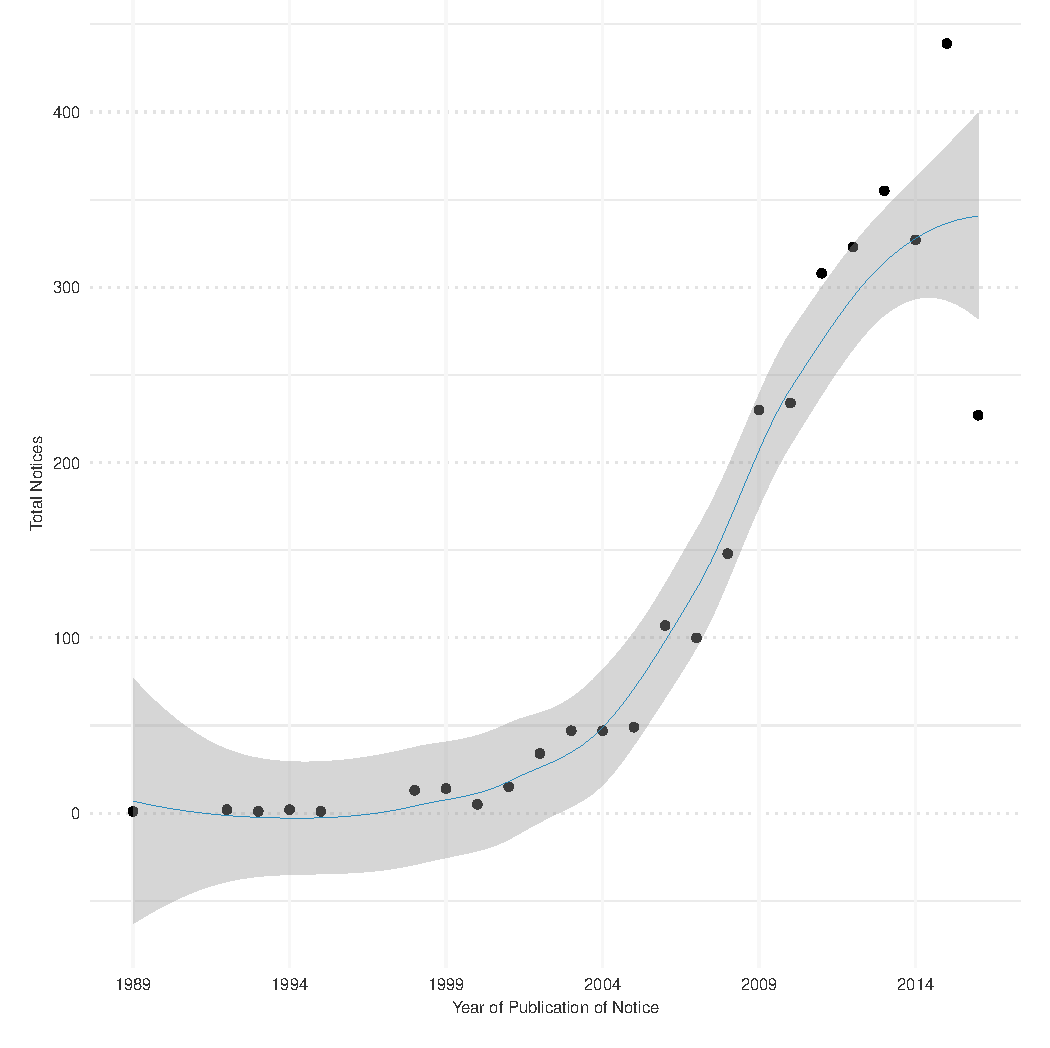
\includegraphics[scale=.7]{../figs/n_retraction_notices_by_year.pdf}
\caption{Retraction Notices Per Year}
\label{fig:n_retraction_notices_per_year}
\end{figure}

The rapid rise in the number of retractions shown above is likely the result of a combination of increasing production and improvements in detection. In all, there is an ever faster growing number of articles that should not have been published in the first place.

To understand why the articles are retracted, we coded a random sample of 100 retraction notices. 39\% of the notices mentioned plagiarism as one of the major reasons for retracting the article. (Plagiarism includes self-plagiarism, duplication of data, words, and publishing the same or similar article in multiple journals.) Major errors or fraud contributed to another 51\% of the retractions, with fraud alone contributing to 24\% of the retractions. Ethics violations (2) and conflict over authorship or approval from other authors (5) contributed to the rest. The percentage of retractions attributable to major errors or fraud in our data is similar to the number obtained by other research on reasons for retraction in other corpora. For instance, a study of 1,112 Biomedicine articles retracted between 1997 and 2009 found that 55\% were retracted for some type of misconduct \citep{budd2011retracted} (see also \citet{steen2011retractions}). Articles are mostly retracted because the research cannot be trusted.

These flawed articles often accrue a fair number of citations. In our data, the articles had been cited 39,792 times before being retracted, with another ~34,000 citations and counting after retraction. This is not unsurprising, given that it took, on average, 2.85 years for the article to be retracted. The median time before the article was retracted was two years (see Figure \ref{fig:ttr}) with 28.1\% of the articles taking four or more years to be retracted. These numbers are similar to those obtained elsewhere \citep[e.g.,][]{steen2013has}.

\begin{figure}[H]
\centering
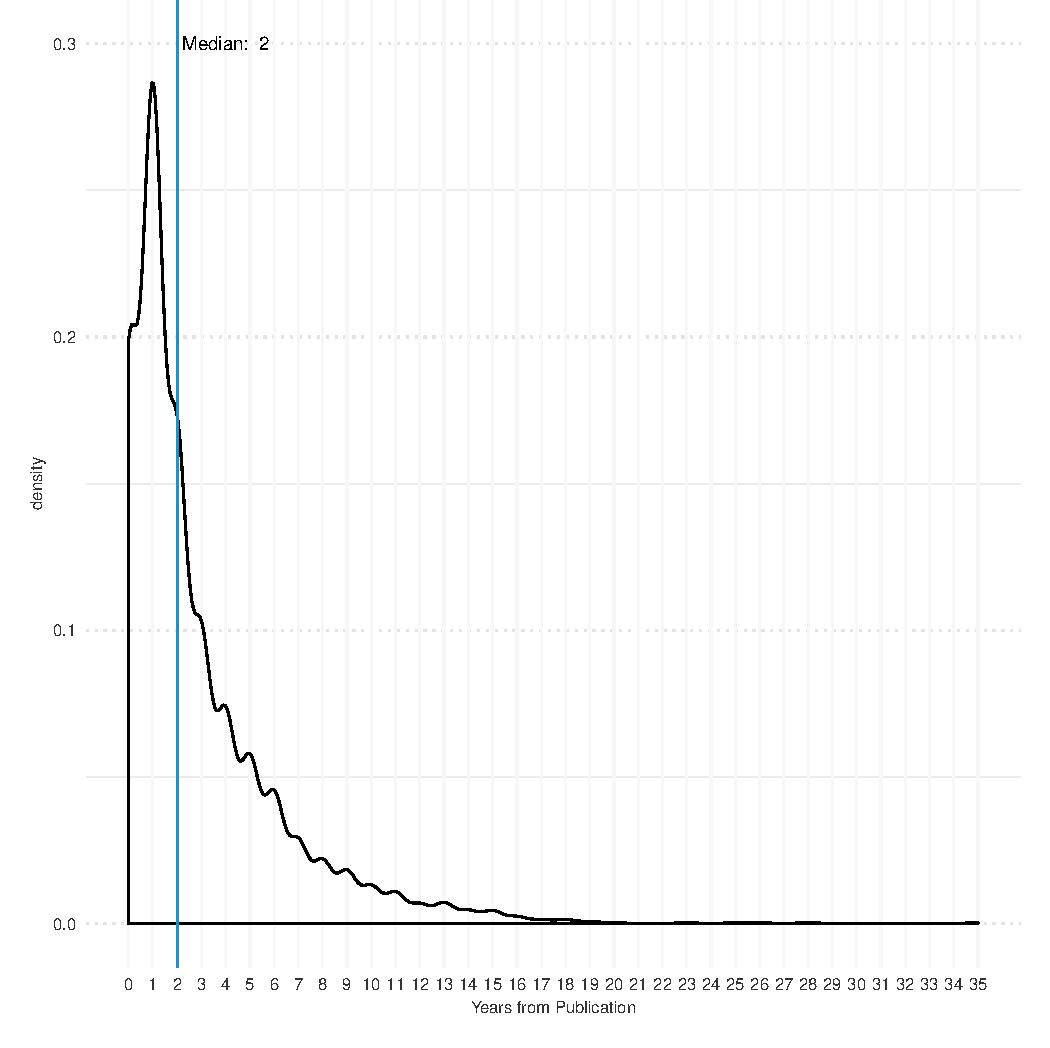
\includegraphics[scale=.7]{../figs/time_to_retraction.pdf}
\caption{Time to Retraction}
\label{fig:ttr}
\end{figure}

To investigate a secondary question of whether the greater readership of more prominent journals would mean that problematic articles are flagged more quickly, we estimated the relationship between the Journal Impact Factor (JIF) and average time to retraction. As Figure \ref{fig:jif_ttr} shows, the relationship is flat---flawed articles in low ranked journals are retracted about as quickly as flawed articles in higher-ranked journals.

\begin{figure}[H]
\centering
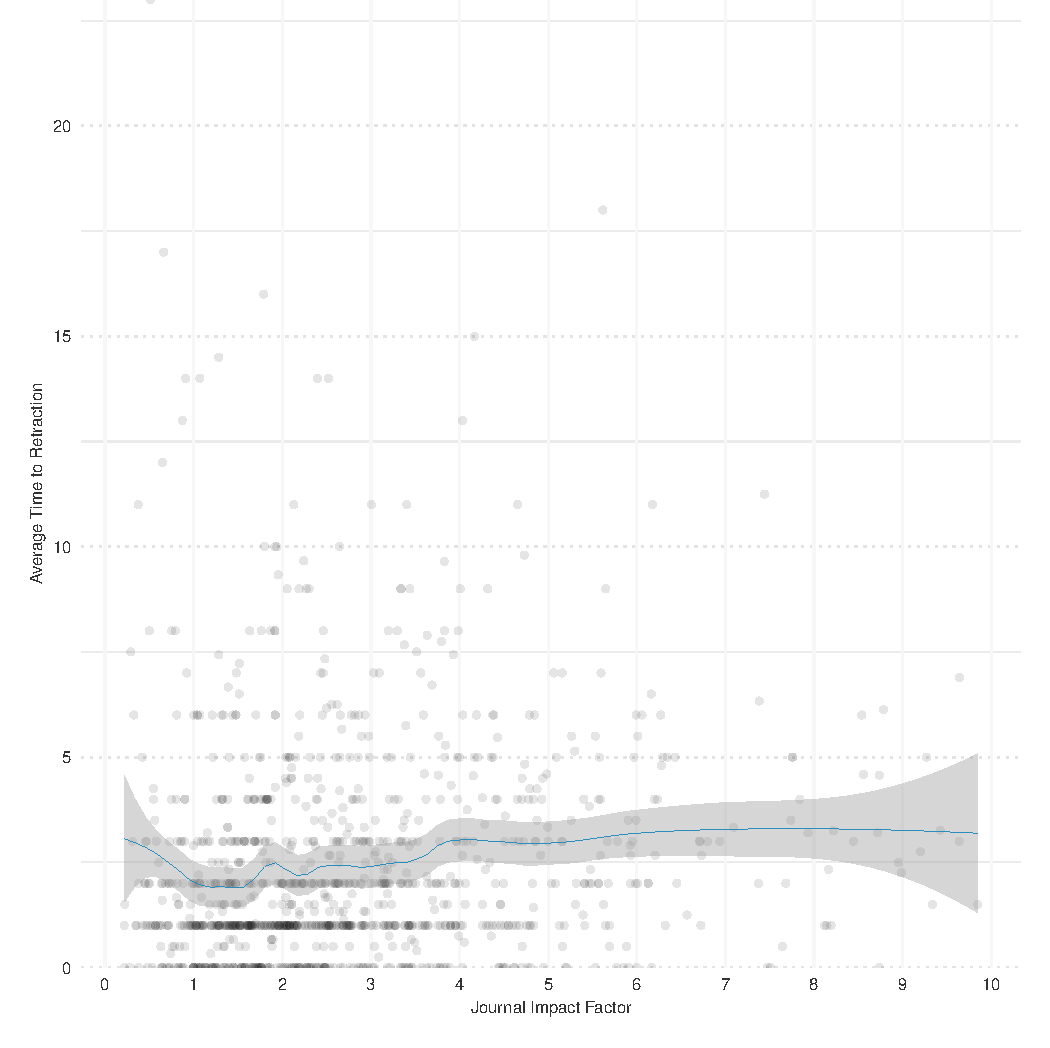
\includegraphics[scale=.7]{../figs/jif_time_to_retraction.pdf}
\caption{Relationship Between Journal Impact Factor and Time to Retraction}
\label{fig:jif_ttr}
\end{figure}

Given that most retracted articles are retracted because of serious error or fraud, we expect retracted articles to \textit{never} be cited without acknowledgment of the problem a year or more---taking account of long publication windows---after the retraction notice has been published. However, retracted articles were cited another 22,932 times between the year after they were retracted and August 2016.\footnote{\ref{code_pre_post} presents some robustness checks based on how we used data on our database to code what is pre- and post- retraction. We manually coded 300 articles to estimate measurement error and found that error plausibly leads to a small (.5\%) \textit{reduction} in the proportion of citations we code as post-publication.} Thus, on average, the retracted articles received an additional 7.5 citations. Given the skew in retraction notices, with the bulk being published in recent years, these totals include very little post retraction data for many of the articles. In other words, the results are a \textit{lower bound} of the percentage of citations that likely happen after an article has been retracted.

To explore the frequency of citations before and after retraction, we plotted line graphs of total citations per article per year against year from the publication of retraction notice (see Figure \ref{fig:pre_post_retraction}). We overlaid the lines with the median number of citations per article per year. We limit ourselves to 10 years before and after the publication of the retraction notice as the data are very sparse beyond that. Total citations decline when the retraction notice is published---the median goes from 3 to 2 between the year the retraction notice is published and the next year, followed by a plateauing.

\begin{figure}[H]
\centering
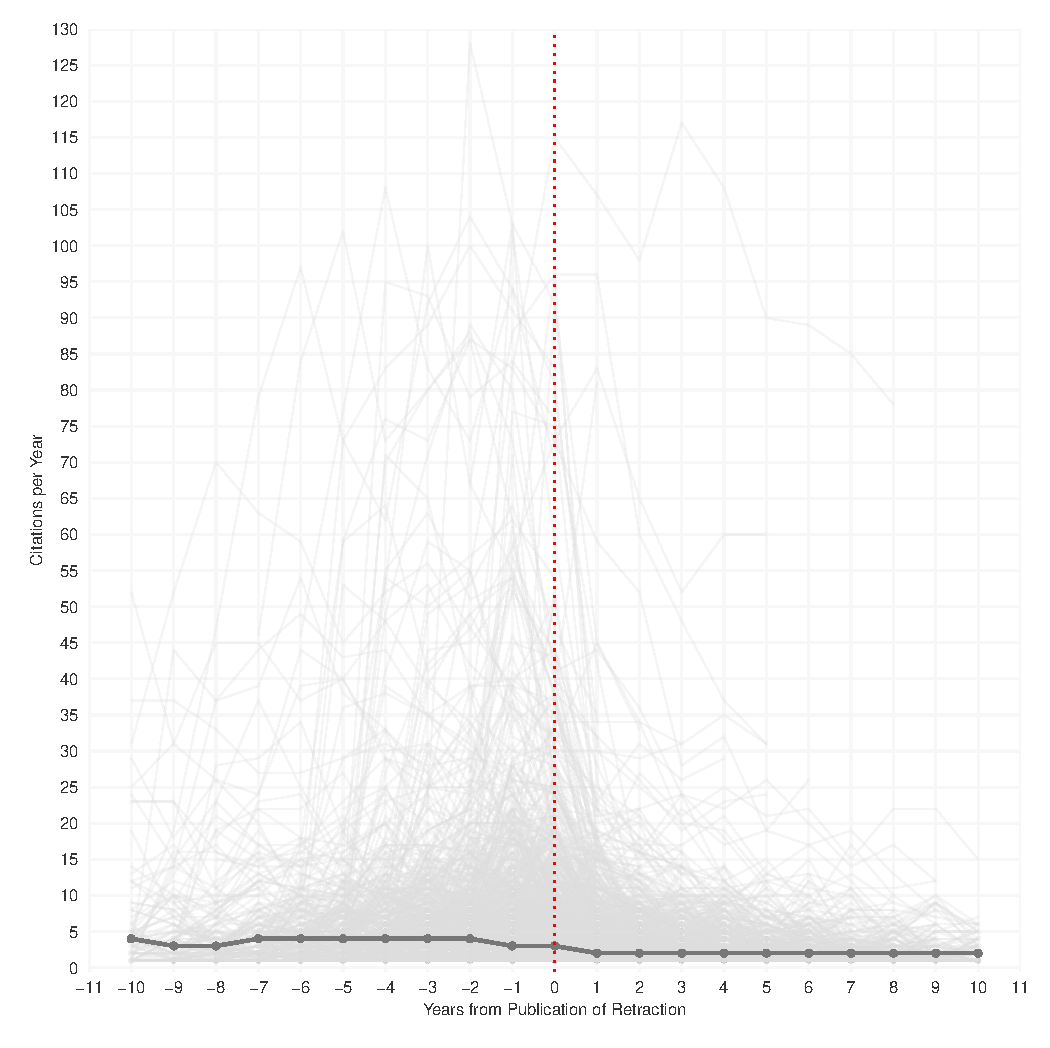
\includegraphics[scale=.7]{../figs/retracted_growth_curve.pdf}
\caption{Number of Citations to Retracted Articles per Year}
\label{fig:pre_post_retraction}
\end{figure}

Figure \ref{fig:pre_post_retraction} elides over the fact that we do not observe data on all articles over all the plotted years after the publication notice. For instance, if the retraction notice was published in 2014, we only observe one more full year of citations---2015. Thus, to look more formally at the impact of the publication of retraction notices a year, two years, and three years after, we create subsets of data where we have all the articles for which we have at least one year, two years, and three years worth of data after the publication of the retraction notice. To analyze these subsets, we regress the number of citations per year per article on years to retraction notice (to account for any linear time trend), a dummy for 1-, 2-, and 3- years after the publication of the retraction notice and an interaction between the two. We cluster the standard errors by article to account for the fact that we have multiple observations per article. Letting $i$ iterate over articles and $j$ iterate over years in which citations are made, letting $y_{ij}$ denote citations received by article $i$ in year $j$, $t_i$ denote years to retraction of article $i$, $d_i$ denote a dummy for transition (1-, 2-, and 3- years after the retraction notice), $\alpha_i$ denote fixed effect for each article, and $\sigma_i$ capture within article correlation in $y_i$ across $j$, we estimated the following set of equations:

\begin{align}
\label{eqn:eqn1}
y_{ij} \sim N(\beta_1 t_i+ \beta_2 d_i + \beta_3 (t_i * d_i) + \alpha_i; \sigma^2_{\epsilon})\\ \nonumber
\alpha_i \sim N(0, \sigma^2_{\alpha_i})
\end{align}

The results of the model can be seen in Table \ref{tab:tab2}. As Table \ref{tab:tab2} shows, on average an article is cited about 5--6 times per year in the year the retraction notice is published. When considering distance from retraction we see that one, two, and three years later, an average article accrues about two fewer citations per year, a drop that is statistically and substantively significant. There is also a small negative slope in the number of citations per year for models that estimate the effect one and two years out. So the number of citations is slowly decreasing but we can comfortably reject the notion that citation rate post publication of the retraction notice is zero.


% Table created by stargazer v.5.2.2 by Marek Hlavac, Harvard University. E-mail: hlavac at fas.harvard.edu
% Date and time: Fri, Feb 05, 2021 - 9:49:48 AM
% Requires LaTeX packages: dcolumn 
\begin{table}[!htbp] \centering 
  \caption{Impact of Publication of Retraction Notice on the Number of Times Retracted Articles Are Cited per Year} 
  \label{tab:tab2} 
\begin{tabular}{@{\extracolsep{5pt}}lD{.}{.}{-1} D{.}{.}{-1} D{.}{.}{-1} } 
\\[-1.8ex]\hline 
\hline \\[-1.8ex] 
 & \multicolumn{3}{c}{\textit{Dependent variable:}} \\ 
\cline{2-4} 
\\[-1.8ex] & \multicolumn{3}{c}{Citations Per Year} \\ 
 & \multicolumn{1}{c}{1 Year Later} & \multicolumn{1}{c}{2 Years Later} & \multicolumn{1}{c}{3 Years Later} \\ 
\\[-1.8ex] & \multicolumn{1}{c}{(1)} & \multicolumn{1}{c}{(2)} & \multicolumn{1}{c}{(3)}\\ 
\hline \\[-1.8ex] 
 (1, 2, 3) Years After Notice & -2.4^{***} & -2.1^{***} & -1.9^{***} \\ 
  & (0.2) & (0.2) & (0.3) \\ 
  Years to Notice & -0.01 & -0.2^{***} & -0.3^{***} \\ 
  & (0.03) & (0.03) & (0.03) \\ 
  (1, 2, 3) Years After Notice*Years to Notice & -0.4^{***} & -0.2^{***} & 0.002 \\ 
  & (0.04) & (0.05) & (0.1) \\ 
  Constant & 6.0^{***} & 5.2^{***} & 4.7^{***} \\ 
  & (0.2) & (0.1) & (0.2) \\ 
 \hline \\[-1.8ex] 
Observations & \multicolumn{1}{c}{12,511} & \multicolumn{1}{c}{11,486} & \multicolumn{1}{c}{10,428} \\ 
Akaike Inf. Crit. & \multicolumn{1}{c}{83,835.6} & \multicolumn{1}{c}{76,511.3} & \multicolumn{1}{c}{69,534.9} \\ 
Bayesian Inf. Crit. & \multicolumn{1}{c}{83,880.2} & \multicolumn{1}{c}{76,555.4} & \multicolumn{1}{c}{69,578.4} \\ 
\hline 
\hline \\[-1.8ex] 
\textit{Note:}  & \multicolumn{3}{r}{$^{*}$p$<$0.1; $^{**}$p$<$0.05; $^{***}$p$<$0.01} \\ 
\end{tabular} 
\end{table} 


We conducted multiple robustness tests. Table ~\ref{tab:non_linear} presents results of a model where we control for non-linear time trends---squared and cubic polynomial terms for time to retraction. And Table ~\ref{tab:poisson} presents results of a poisson model with the same structure. A careful look at the tables underlines the conclusions from Table \ref{tab:tab2} and Figure \ref{fig:pre_post_retraction}---there is a small decline post the publication of retraction notice but citations to retracted articles continue post retraction. 

To estimate how many of the citations after retraction are \textit{fail to acknowledge problems}, we coded a random sample of 100 articles that cited a retracted article pre-retraction and 275 articles that cited retracted research a year or more after the publication of the retraction notice. We could not locate 32 articles, leaving us with 343 total articles. There were no false positives. Of the 87 articles citing retracted articles before or in the same year the retraction notice was published, 85 (97.7\%) did not acknowledge any problems with the research being cited. Of the 256 articles citing retracted articles the year after the retraction notice was published, 234 (91.4\%) were did not mention problems - a slight trend downward. (Figure \ref{fig:prop_approving_per_year} plots the proportion of citations failing to acknowledge problems by year.) In all, the data suggest that retracted articles continue to be cited at non-zero rates after retraction and they are still very much failing to acknowledge concerns.

\begin{figure}
\centering
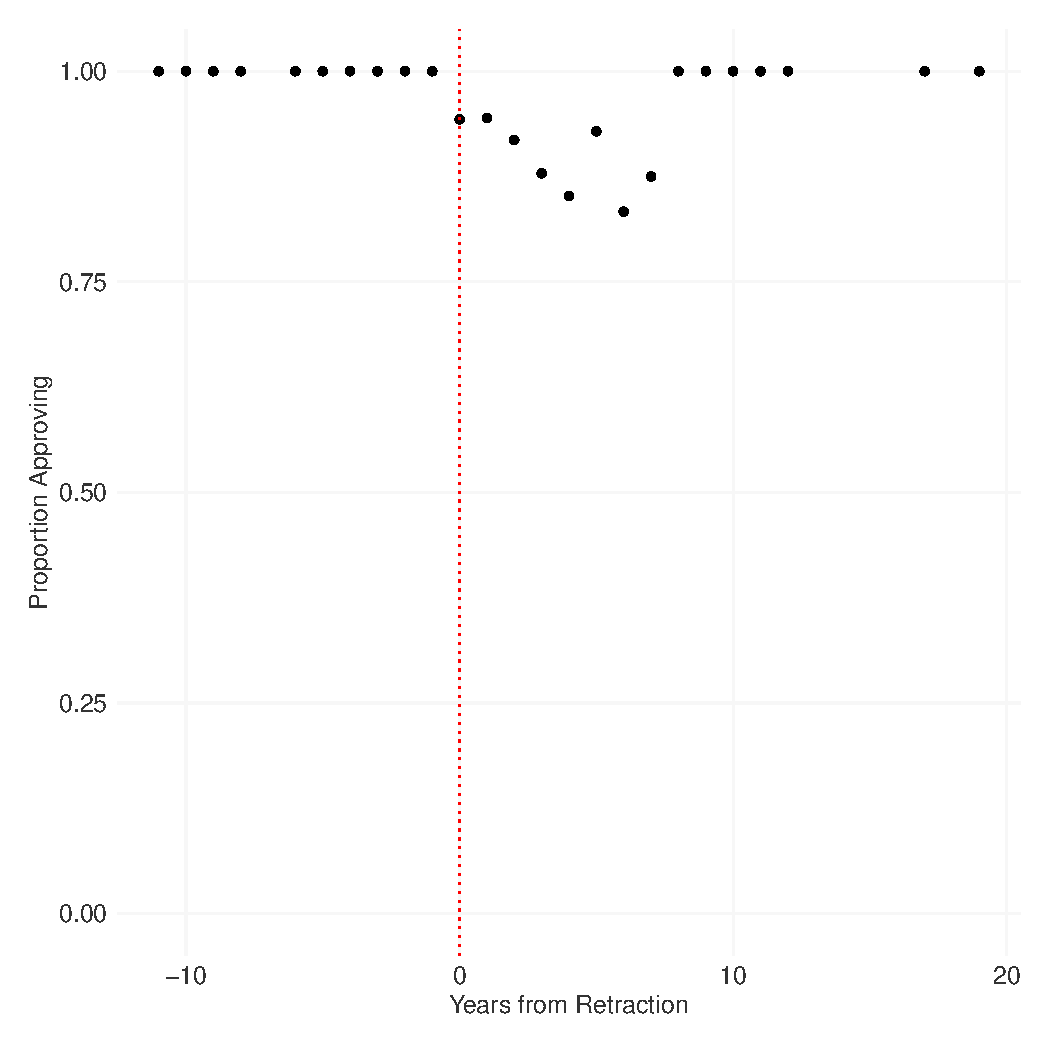
\includegraphics[width=10cm]{../figs/pre_post_prop_approving.pdf}
\caption{Proportion of Citations That Fail to Acknowledge Problems Per Year}
\label{fig:prop_approving_per_year}
\end{figure}

\subsection{Citations Before and After Publication of Nieuwenhuis et al.}

Prima facie evidence suggests little impact of the publication of \citet{nieuwenhuis2011} on citations to articles mistaking the difference between significant effect and insignificant effect as evidence for a significant difference. In the two years before the publication of \citet{nieuwenhuis2011}, and the year \citet{nieuwenhuis2011} was published (2011), the 79 articles making the mistake were cited 2,267 times. Between 2012 and 2015, the articles were cited an additional 6,604 times.

Figure \ref{fig:niewenhuis} offers a closer look. It plots the total number of citations received per year by each of the papers making the mistake, the average number of citations received per year by articles making the mistake, and smoothed \texttt{loess} growth curves. The plot also shows there is a skew in citation rates (skewness based on the method of moments = 2). To account for the skew, we switched means with medians. Doing so yields a pretty similar pattern except for the expected intercept shift (see Figure \ref{fig:median_niewenhuis}). Not all articles making the error, however, have results similarly affected by the error. Fortunately, \citet{nieuwenhuis2011} flag articles where the error has potentially serious consequences for the results. Thus, next, we track what happens to citations to such articles. We track how the median number of citations vary across years and whether they are affected by the publication of the \citet{nieuwenhuis2011}. As Figure \ref{fig:serious_niewenhuis} shows, the median number of citations steadily and modestly increase over time with the publication of \citet{nieuwenhuis2011}.

\begin{figure}[H]
\centering
 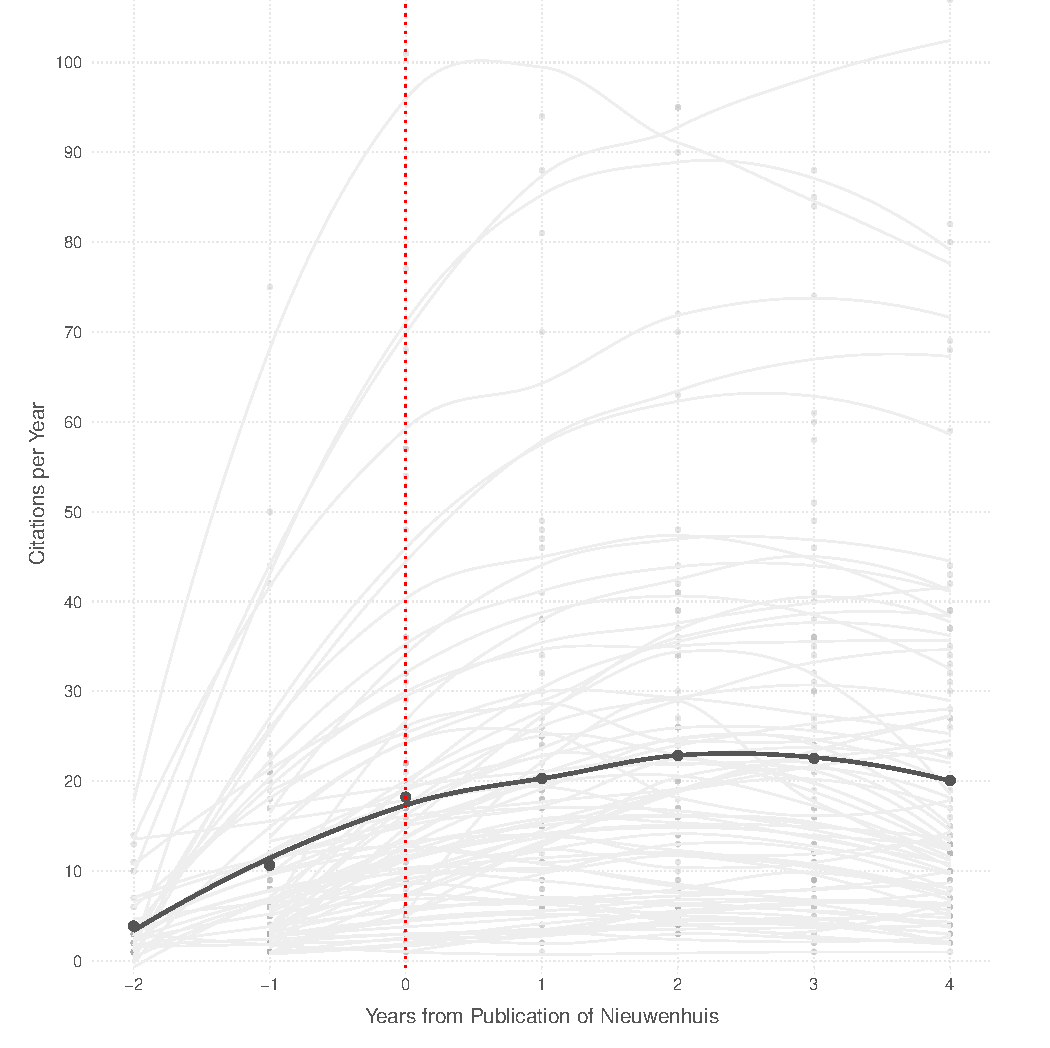
\includegraphics[scale=.7]{../figs/nw_growth_curve.pdf}
 \caption{Number of Citations to Articles Containing the Error Per Year}
 \label{fig:niewenhuis}
\end{figure}

To estimate the percentage of citations that do not acknowledge problems after the publication of Nieuwenhuis et al., we coded whether the citation acknowledged the problem or not in 100 randomly chosen articles citing articles with the mistake (see SI \ref{approving_or_not} for further details about how the citations were coded.) Of the 100, only one article noted concerns with the cited article, citing \citep{nieuwenhuis2011} for support.

To more formally explore the change in citation rate as a consequence of the publication of \citet{nieuwenhuis2011}, we regress citations per year on a dummy for the year \citet{nieuwenhuis2011} was published, a linear time trend, and fixed-effect for the article. We also cluster by articles to account for multiple observations per article. In effect, we are estimating an average of within article changes after regressing out a linear time trend as above. Results show, if anything, a modest uptick in citations after \citet{nieuwenhuis2011} is published---a year after the publication of \citet{nieuwenhuis2011}, articles containing the error get about four more citations per year compared to what they were getting before it (see Table \ref{tab:si_tab1}).

Our main analysis for the \citeauthor{nieuwenhuis2011} data is a Difference-in-Differences (DID) analysis. DID gives us a better way to control for over time trends. We estimated whether the difference in citation rates of articles making the error and those not making the error changed after the publication of \citet{nieuwenhuis2011}. In particular, letting $i$ index articles and $j$ index years, we regressed citations per year ($y_ij$) on whether or not the article makes the error ($s_i$), years to the publication of \citeauthor{nieuwenhuis2011} ($n_i$) and an interaction between the two. Again, we clustered the standard errors by article. In all, we estimated the following model:

\begin{align}
\label{eqn:eqn2}
y = \alpha + \beta_1 n_i + \beta_2 s_i + \beta_3 (n*s) + \epsilon
\end{align}

Table \ref{tab:tab1} tabulates the results. Models (1), (3), and (5) define error as all articles making the error. Models (2), (4), and (6) refer to error as articles making ``potentially serious errors.'' As the table shows, 1 or 2 years after \citet{nieuwenhuis2011}, articles making the error were being cited more frequently vis-\`a-vis articles not making the error (Diff. $\sim$ 3). Three years out, we cannot still reject the 0, suggesting that there is no evidence of a decline. For articles making ``potentially serious errors'', the story is much the same, except that the one and two-year out estimates are closer to 3.5 additional citations per year than 3. Three years later, we still cannot say that the articles making ``potentially serious errors'' were being cited any less frequently.  In all, there is strong evidence that citations that do not acknowledge problems remain common after the error is publicized. The publicity of \citeauthor{nieuwenhuis2011} has had little impact, with articles containing errors still being highly cited. These articles may be especially susceptible to continued citations because the nature of the error results in an inference of a difference in differences that is something other researchers are looking for evidence of in order to support an important point.


% Table created by stargazer v.5.2.2 by Marek Hlavac, Harvard University. E-mail: hlavac at fas.harvard.edu
% Date and time: Fri, Aug 03, 2018 - 1:38:56 PM
% Requires LaTeX packages: dcolumn rotating 
\begin{sidewaystable}[!htbp] \centering 
  \caption{Difference-in-Difference Analysis of the Impact of Publication of Nieuwenhuis on the Number of Times per Year Articles Containing the Error Are Cited Vis-a-Vis Articles that Didn't Contain the Error} 
  \label{tab:tab1} 
\small 
\begin{tabular}{@{\extracolsep{5pt}}lD{.}{.}{-1} D{.}{.}{-1} D{.}{.}{-1} D{.}{.}{-1} D{.}{.}{-1} D{.}{.}{-1} } 
\\[-1.8ex]\hline 
\hline \\[-1.8ex] 
 & \multicolumn{6}{c}{\textit{Dependent variable:}} \\ 
\cline{2-7} 
\\[-1.8ex] & \multicolumn{6}{c}{Citations per year} \\ 
 & \multicolumn{2}{c}{1 year out} & \multicolumn{2}{c}{2 years out} & \multicolumn{2}{c}{3 years out} \\ 
\\[-1.8ex] & \multicolumn{1}{c}{(1)} & \multicolumn{1}{c}{(2)} & \multicolumn{1}{c}{(3)} & \multicolumn{1}{c}{(4)} & \multicolumn{1}{c}{(5)} & \multicolumn{1}{c}{(6)}\\ 
\hline \\[-1.8ex] 
 Treatment Date & 7.2^{***} & 7.7^{***} & 5.1^{***} & 5.5^{***} & 3.7^{***} & 3.9^{***} \\ 
  & (0.9) & (0.7) & (0.9) & (0.7) & (1.0) & (0.8) \\ 
  Error or Not & 1.5 & 0.004 & 2.1 & 0.6 & 2.8 & 1.6 \\ 
  & (2.5) & (2.8) & (2.4) & (2.7) & (2.4) & (2.6) \\ 
  Makes Error*Treatment Date & 3.1^{**} & 3.7^{***} & 2.7^{**} & 3.5^{***} & 1.7 & 2.1 \\ 
  & (1.2) & (1.3) & (1.2) & (1.3) & (1.3) & (1.5) \\ 
  Constant & 9.5^{***} & 10.2^{***} & 11.7^{***} & 12.6^{***} & 13.1^{***} & 14.0^{***} \\ 
  & (1.8) & (1.5) & (1.7) & (1.5) & (1.7) & (1.4) \\ 
 \hline \\[-1.8ex] 
Observations & \multicolumn{1}{c}{957} & \multicolumn{1}{c}{957} & \multicolumn{1}{c}{957} & \multicolumn{1}{c}{957} & \multicolumn{1}{c}{957} & \multicolumn{1}{c}{957} \\ 
Akaike Inf. Crit. & \multicolumn{1}{c}{7,328.2} & \multicolumn{1}{c}{7,327.8} & \multicolumn{1}{c}{7,408.8} & \multicolumn{1}{c}{7,407.5} & \multicolumn{1}{c}{7,474.9} & \multicolumn{1}{c}{7,475.2} \\ 
Bayesian Inf. Crit. & \multicolumn{1}{c}{7,357.4} & \multicolumn{1}{c}{7,357.0} & \multicolumn{1}{c}{7,437.9} & \multicolumn{1}{c}{7,436.7} & \multicolumn{1}{c}{7,504.0} & \multicolumn{1}{c}{7,504.4} \\ 
\hline 
\hline \\[-1.8ex] 
\textit{Note:}  & \multicolumn{6}{l}{$^{*}$p$<$0.1; $^{**}$p$<$0.05; $^{***}$p$<$0.01} \\ 
 & \multicolumn{6}{l}{Models (1), (3), and (5) define error as any article making the error.} \\ 
 & \multicolumn{6}{l}{And Models (2), (4), and (6) refer to error as articles making ``potentially serious errors.''} \\ 
\end{tabular} 
\end{sidewaystable} 


\section{Discussion}
Only some of the points in a scientific paper rely on original work. For most points, scientists rely on work done by others. For instance, scientists rely on other research to buffet arguments, situate work in a research tradition, credit others for original arguments, data, and results, etc. \citep{erikson2014taxonomy}. However,  sometimes, the work done by others is problematic. For instance, sometimes, the claims in the cited work are not only wrong but made with fraudulent data. And we expect scientists to either not refer to such work or acknowledge the issues fully, especially after the errors have been publicized.

In this paper, we use a large dataset of retracted articles and their citations and a novel dataset of articles with a statistical error and their citations and discover that the citation rate to problematic research after publication of problems is lower but still significant. We also find that citations that fail to acknowledge problems with problematic cited work are common years after the articles have been retracted.

We have a few hypotheses (but no data) about why these types of citations exist. One shallow reason is that journal publishers do not seem to screen citations to retracted research in submitted manuscripts. Instead, they assume that scientists will cite appropriately and that the peer review process will screen the remaining problems. 

Another potential reason is that scientists do not scrutinize the articles they cite. One reason for that is that they trust published work. Their trust is likely buffeted by the belief that scientific misconduct is limited to a few bad people, which in turn may be driven by the fact that media reporting often focuses on personalities rather than processes. For example, cases of Diederik Stapel, who fabricated data behind at least 30 papers \citep{levelt2012flawed}, John Darsee, who faked data behind nearly 100 publications \citep{stewart1987integrity, anderson2013research, wallis1983fraud}, and Jan Hendrik Sch{\"o}n, who during a period in 2001 published a research paper every eight days based on fabricated data \citep{service2003scientific, anderson2013research} were heavily covered in the media. So were the cases of Andrew Wakefield, who published an article linking MMR vaccine to autism using fabricated data \citep{wakefield1998retracted, deer2011case, godlee2011wakefield}, and recently Michael Lacour, who published a paper in \textit{Science} based on fabricated data \citep{broockman2015irregularities, mcnutt2015editorial}.\footnote{Other prominent cases include that of William Summerlin, who painted mice rather than transplant skin \citep{basu2006they, anderson2013research}, Woo Suk Hwang, who claimed to have cloned embryos, Eric Poehlman, who fabricated data behind at least ten papers and numerous grant applications.} Each of these cases was framed as an example of misconduct by a bad actor, the subtext often being that a bad actor is an outlier.

Misconduct, however, is not limited to a few bad actors.  A large anonymous survey of early- and mid-career scientists found that about 2\% of scientists admitted to engaging in fabricating, falsifying, or plagiarizing in the last \textit{three} years \citet{martinson2005scientists} (see also \citet{titus2008repairing}). Another study found that nearly 34\% of the respondents in past surveys admitted to engaging in questionable research practices \citet{fanelli2009many}.

The other likely reason for trust in peer-reviewed research is that the rate of official retractions is extremely low. For instance, in a study of the nearly 9.4 million articles published between 1950 and 2004 and available on PubMed, only 596 had been retracted \citep{cokol2007many}. In all likelihood, however, the actual rate of serious errors in manuscripts is manifolds that rate. For instance, \citet{cokol2007many} estimate the rate at which articles ought to be retracted to be anywhere between 16.7 times to 167.8 times the actual rate. And these estimates do not account for research that involves harder-to-prove malpractice such as filing away non-significant results \citep{franco2014publication}, conducting specification searches, and other more fundamental concerns like low power, which reduces the likelihood that a nominally statistically significant finding reflects a true effect \citep{button2013power, ioannidis2005most}. 

It is also likely that scientists cite erroneous research due to a lack of time stemming from the pressure to publish. Some scientists may also buckle to incentives to treat published research generously, given harsh (but accurate) judgments may provoke some reviewers. More generally, peer reviews tend to focus on instances where the authors fail to cite someone or miss the journal's formatting requirements more than concerns over incorrectly citing bad research. This means that there is little incentive to cite carefully.

Static reference databases likely exacerbate the problem. While publisher databases are quick to mark papers as retracted, many researchers rely on static reference databases stored on their computers for citations. These databases sometimes contain articles that have since been retracted. For instance, \citet{davis2012persistence} finds that personal Mendeley libraries contained 1,340 retracted articles. In all, there are many reasons why scientists may cite erroneous research, even after the errors have been publicized via a retraction notice or an article noting the problem.

These 'miscitations' are avoidable. Improving how the information about problematic research is generated and communicated can ameliorate the problem. For example, our study has resulted in the creation of a relatively large database of retracted research. Other groups are compiling even larger databases (see Retractionwatch.com's \href{http://retractiondatabase.org/}{retraction database}). These databases can be leveraged by publishers to screen submitted manuscripts for citations to retracted research. They could also be used to develop web browser add-ons for scholarly search engines such as Google Scholar and JSTOR to highlight problematic articles listed on a web page. In addition, tools that automatically create pull requests to personal bibliography libraries posted on open publication platforms like GitHub could be built. Taking steps like these should lead to significant improvements in reducing citations of problematic research.

To conclude, this study contributes to a rich literature on scholarly citation behavior. For example, \citet{rekdal2014academic} introduces the concept of \textit{academic urban legends}--- rumors that appear frequently and in complex and colorful ways that can usually be traced back to poorly employed sources---like the story of a decimal point error resulting in the belief that spinach is a good source of iron. Similarly, \citet{lance2006sources} explores the basis for \textit{methodological urban legends} in the form of four commonly employed criteria for the goodness of fit indices, reliability, interrater agreement indices, and eigenvalues. They find that much of the hype about these criteria has emerged from an inappropriate citation of the source material. By the same token, \citet{harzing2002our} examined the citation network of 60 references on expatriate failure rates (EFRs)---the phenomenon of an expatriate returning home before their contractual period of employment expires. He finds that one reference was cited 22 times, with only six correctly representing the EFRs reported in the original work. Similarly, \citet{todd2010one} report that of 198 randomly selected citations to articles in two recent issues of 33 marine biology journals, 1 in 4 represented an inappropriate citation---ambiguous, no support, or empty (citation to a secondary source).

We find that citations to problematic research are only modestly impacted by the publication of retraction notifications or other articles that highlight major errors. We also find that the rate at which researchers cite problematic articles without acknowledging problems after the problem has been publicized remains high.  


\clearpage
\bibliographystyle{rss}
\bibliography{error}

\clearpage
\appendix
\renewcommand{\thesection}{SI \arabic{section}}
\renewcommand\thetable{\thesection.\arabic{table}}
\renewcommand\thefigure{\thesection.\arabic{figure}}
\counterwithin{figure}{section}
\setcounter{figure}{0}
\setcounter{section}{0}
\setcounter{table}{0}

\begin{center}
\Large{Supporting Information}
\end{center}

\section{Classifying Citations as Post-Retraction or Not}
\label{code_pre_post}
A few retraction notices, retracted articles, and articles citing the retracted articles have earlier online (or conference) publication dates than the print publication dates recorded by WoS. As a result, post-retraction citations can be classified as otherwise. Or vice versa. To determine the impact of this issue and issues like these on our estimate of the lower bound of the proportion of citations that are made a year or more after the publication of the retraction notice, we manually recorded the online publication dates for a random sample of 300 citations to retracted articles, the associated retraction notices, and retracted articles. We could not retrieve 20 articles citing a retracted article.  Of the remaining 280 records, switching to online publication dates suggests that three articles were misclassified as post-retraction (2.2\%) and four were misclassified as not post-retraction (3.2\%). Taking these error rates at their face value, we re-calibrated our results. The recalibration results in an increase in the number of post-retraction citations, from 22,932 to 23,289. Or, the lower bound of the proportion of citations that happen the year after the retraction notice is published goes from 31.2\% to 31.7\%.

\section{Coding Citations as Acknolwedging Problems Or Not}
\label{approving_or_not}
To code the citations, we downloaded citing articles and their associated retracted article. A research assistant then edited the citing article pdf to highlight where the retracted article was discussed in the citing article. The judgment of whether the article noted any concerns was made based on a review of the original retracted article pdf and the highlighted text. 

If an article did not note any concerns with the cited article, it was coded as \textit{not acknoledging problems}. Simply disagreeing with the conclusions of an article without noting any concern still meant that the article was being cited in a way that suggests that its findings are trustworthy and were also coded as \textit{not acknowledging problems}. We code articles that note any concern with the citing article, even those unrelated to the cause of retraction, as \textit{acknowledging problems}. 

In the Nieuwenhuis data, we could not locate one of the 100 articles, leaving us with 99 articles. Of the 99 articles, 2 were false positives---the articles did not cite erroneous research, but instead cited a paper with authors and title similar to published erroneous research. Of the 97 remaining articles, only one article noted concerns while citing an article making a mistake, citing \citet{nieuwenhuis2011} for support. 

In the retracted article data, we could not locate 32 articles, leaving us with 343 articles. There were no false positives. Of the 87 articles citing retracted articles before or in the same year the retraction notice was published, 85 (97.7\%) did not acknowledge problems. And of the 256 articles citing retracted articles the year after the retraction notice was published, 234 (91.4\%) did not acknowledge problems.

We evaluated the reliability of the coding by having an independent rater code 50 randomly selected citing articles. The two sets of independent codes were found to agree in all 50 instances.

\clearpage

\section{Rate of Citations Before and After Publication of Nieuwenhuis et al.}

\begin{figure}[H]
\centering
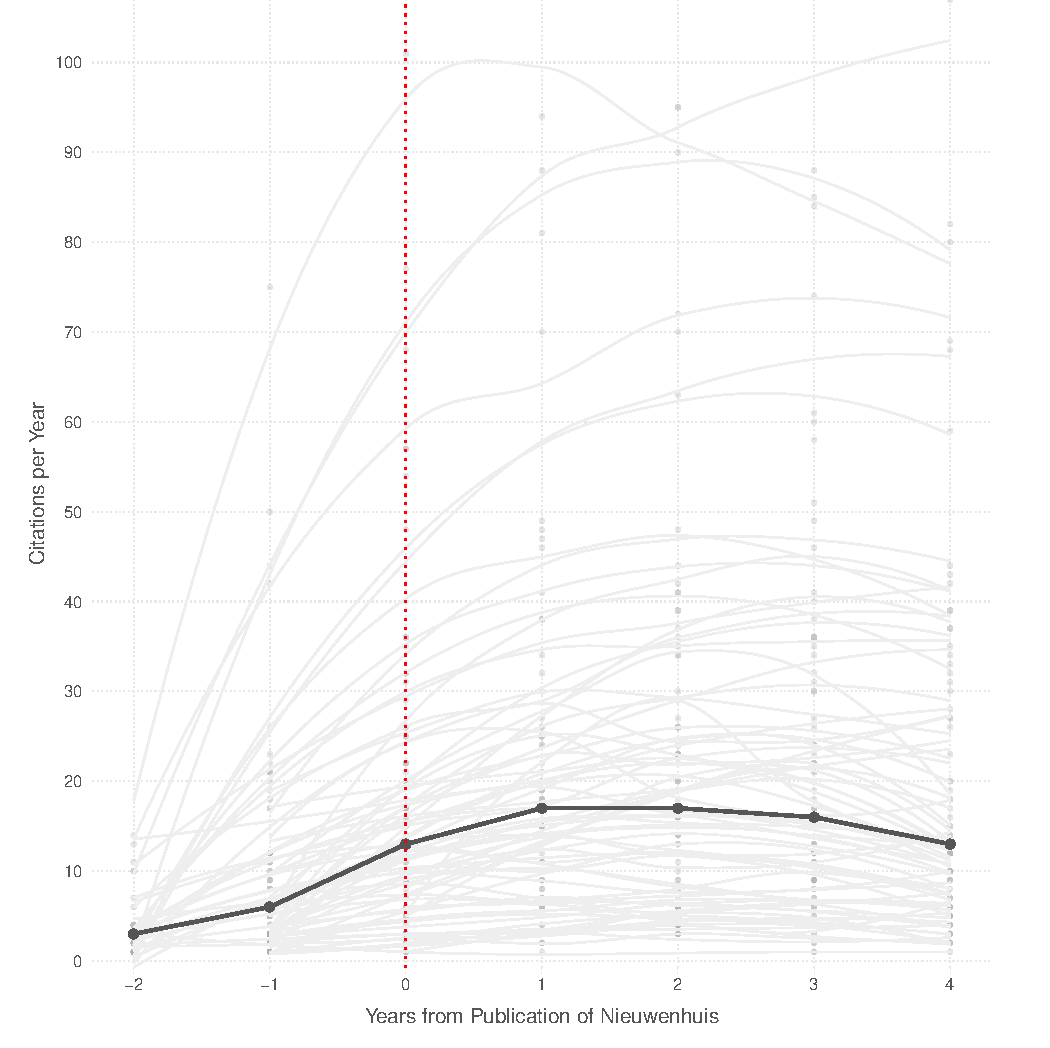
\includegraphics[scale=.7]{../figs/nw_median_growth_curve.pdf}
\caption{Total number of citations received per year by each of the papers making the mistake, and the median number of citations received per year by the articles.}
\label{fig:median_niewenhuis}
\end{figure}

\clearpage
\begin{figure}[H]
\centering
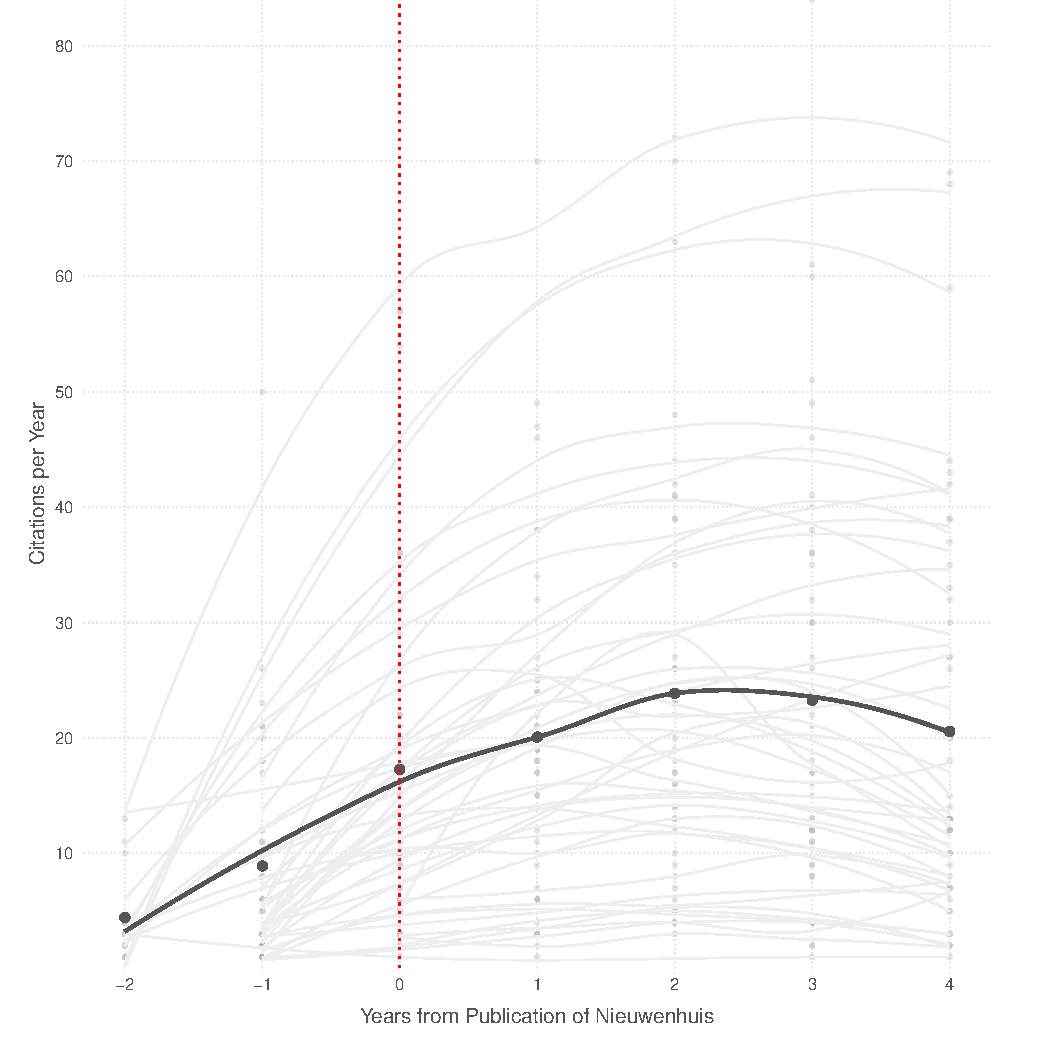
\includegraphics[scale=.7]{../figs/serious_nw_growth_curve.pdf}
\caption{Total number of citations received per year by articles making the mistake with `potentially serious' consequences for the results, and the average number of citations received per year by the articles.}
\label{fig:serious_niewenhuis}
\end{figure}

\clearpage

% Table created by stargazer v.5.2.2 by Marek Hlavac, Harvard University. E-mail: hlavac at fas.harvard.edu
% Date and time: Fri, Aug 03, 2018 - 1:38:47 PM
% Requires LaTeX packages: dcolumn 
\begin{table}[!htbp] \centering 
  \caption{Change in the Number of Citations to Articles Containing the Error Per Year Before and After Publication of Nieuwenhuis} 
  \label{tab:si_tab1} 
\begin{tabular}{@{\extracolsep{5pt}}lD{.}{.}{-1} D{.}{.}{-1} } 
\\[-1.8ex]\hline 
\hline \\[-1.8ex] 
 & \multicolumn{2}{c}{\textit{Dependent variable:}} \\ 
\cline{2-3} 
\\[-1.8ex] & \multicolumn{2}{c}{Citations Per Year} \\ 
 & \multicolumn{1}{c}{All Articles with Mistakes} & \multicolumn{1}{c}{Articles with Potentially Serious Errors} \\ 
\\[-1.8ex] & \multicolumn{1}{c}{(1)} & \multicolumn{1}{c}{(2)}\\ 
\hline \\[-1.8ex] 
 Transition Date & 3.8^{**} & 5.0^{**} \\ 
  & (1.7) & (2.0) \\ 
  Time & 2.0^{***} & 2.1^{***} \\ 
  & (0.4) & (0.5) \\ 
  Constant & 12.4^{***} & 11.6^{***} \\ 
  & (1.9) & (2.1) \\ 
 \hline \\[-1.8ex] 
Observations & \multicolumn{1}{c}{487} & \multicolumn{1}{c}{276} \\ 
Akaike Inf. Crit. & \multicolumn{1}{c}{3,818.0} & \multicolumn{1}{c}{2,095.8} \\ 
Bayesian Inf. Crit. & \multicolumn{1}{c}{3,838.9} & \multicolumn{1}{c}{2,113.9} \\ 
\hline 
\hline \\[-1.8ex] 
\textit{Note:}  & \multicolumn{2}{r}{$^{*}$p$<$0.1; $^{**}$p$<$0.05; $^{***}$p$<$0.01} \\ 
\end{tabular} 
\end{table} 


\clearpage

% Table created by stargazer v.5.2.2 by Marek Hlavac, Harvard University. E-mail: hlavac at fas.harvard.edu
% Date and time: Mon, Feb 15, 2021 - 11:19:58 PM
% Requires LaTeX packages: dcolumn 
\begin{table}[!htbp] \centering 
  \caption{Impact of Publication of Retraction Notice on the Number of Times Retracted Articles Are Cited per Year With Non-Linear Time Trends} 
  \label{tab:non_linear} 
\begin{tabular}{@{\extracolsep{5pt}}lD{.}{.}{-1} D{.}{.}{-1} D{.}{.}{-1} } 
\\[-1.8ex]\hline 
\hline \\[-1.8ex] 
 & \multicolumn{3}{c}{\textit{Dependent variable:}} \\ 
\cline{2-4} 
\\[-1.8ex] & \multicolumn{3}{c}{Citations Per Year} \\ 
 & \multicolumn{1}{c}{1 Year Later} & \multicolumn{1}{c}{2 Years Later} & \multicolumn{1}{c}{3 Years Later} \\ 
\\[-1.8ex] & \multicolumn{1}{c}{(1)} & \multicolumn{1}{c}{(2)} & \multicolumn{1}{c}{(3)}\\ 
\hline \\[-1.8ex] 
 (1, 2, 3) Years After Notice & -2.1^{***} & -2.0^{***} & -2.8^{***} \\ 
  & (0.2) & (0.3) & (0.4) \\ 
  Years to Notice & 0.2^{***} & -0.3^{***} & -0.5^{***} \\ 
  & (0.1) & (0.05) & (0.04) \\ 
  (1, 2, 3) Years After Notice*Years to Notice & 0.02^{***} & -0.002 & -0.02^{***} \\ 
  & (0.004) & (0.004) & (0.005) \\ 
  Years to Notice Squared & 0.000^{***} & 0.000^{**} & 0.000 \\ 
  & (0.000) & (0.000) & (0.000) \\ 
  Years to Notice Cubed & -0.9^{***} & -0.2 & 0.4^{***} \\ 
  & (0.1) & (0.1) & (0.1) \\ 
  Constant & 95.1^{***} & 94.0^{***} & 93.6^{***} \\ 
  & (13.8) & (6.0) & (1.8) \\ 
 \hline \\[-1.8ex] 
Observations & \multicolumn{1}{c}{12,511} & \multicolumn{1}{c}{11,486} & \multicolumn{1}{c}{10,428} \\ 
Akaike Inf. Crit. & \multicolumn{1}{c}{73,247.1} & \multicolumn{1}{c}{67,613.2} & \multicolumn{1}{c}{61,861.3} \\ 
Bayesian Inf. Crit. & \multicolumn{1}{c}{90,628.6} & \multicolumn{1}{c}{82,546.2} & \multicolumn{1}{c}{74,705.0} \\ 
\hline 
\hline \\[-1.8ex] 
\textit{Note:}  & \multicolumn{3}{r}{$^{*}$p$<$0.1; $^{**}$p$<$0.05; $^{***}$p$<$0.01} \\ 
\end{tabular} 
\end{table} 


\clearpage

% Table created by stargazer v.5.2.2 by Marek Hlavac, Harvard University. E-mail: hlavac at fas.harvard.edu
% Date and time: Mon, Feb 15, 2021 - 10:40:31 PM
% Requires LaTeX packages: dcolumn 
\begin{table}[!htbp] \centering 
  \caption{Impact of Publication of Retraction Notice on the Number of Times Retracted Articles Are Cited per Year With Non-Linear Time Trends And Modeled as a Poisson} 
  \label{tab:poisson} 
\begin{tabular}{@{\extracolsep{5pt}}lD{.}{.}{-1} D{.}{.}{-1} D{.}{.}{-1} } 
\\[-1.8ex]\hline 
\hline \\[-1.8ex] 
 & \multicolumn{3}{c}{\textit{Dependent variable:}} \\ 
\cline{2-4} 
\\[-1.8ex] & \multicolumn{3}{c}{Citations Per Year} \\ 
 & \multicolumn{1}{c}{1 Year Later} & \multicolumn{1}{c}{2 Years Later} & \multicolumn{1}{c}{3 Years Later} \\ 
\\[-1.8ex] & \multicolumn{1}{c}{(1)} & \multicolumn{1}{c}{(2)} & \multicolumn{1}{c}{(3)}\\ 
\hline \\[-1.8ex] 
 (1, 2, 3) Years After Notice & -0.3^{***} & -0.4^{***} & -0.8^{***} \\ 
  & (0.04) & (0.1) & (0.1) \\ 
  Years to Notice & 0.04^{***} & -0.04^{***} & -0.1^{***} \\ 
  & (0.01) & (0.01) & (0.01) \\ 
  (1, 2, 3) Years After Notice*Years to Notice & 0.003^{***} & -0.003 & -0.01^{***} \\ 
  & (0.001) & (0.002) & (0.003) \\ 
  Years to Notice Squared & 0.000 & -0.000 & -0.000^{***} \\ 
  & (0.000) & (0.000) & (0.000) \\ 
  Years to Notice Cubed & -0.2^{***} & -0.01 & 0.2^{***} \\ 
  & (0.02) & (0.03) & (0.05) \\ 
  Constant & 5.1^{***} & 4.9^{***} & 4.9^{***} \\ 
  & (0.03) & (0.02) & (0.02) \\ 
 \hline \\[-1.8ex] 
\hline 
\hline \\[-1.8ex] 
\textit{Note:}  & \multicolumn{3}{r}{$^{*}$p$<$0.1; $^{**}$p$<$0.05; $^{***}$p$<$0.01} \\ 
\end{tabular} 
\end{table} 


\end{document}
